\documentclass[a4paper, 14pt]{article} %documentclass [tuy chon]{tenlop}
\usepackage[utf8]{vntex}
\usepackage{titling}
\usepackage{enumerate}
\usepackage{enumitem}
\usepackage{ragged2e}
\usepackage{graphicx}
\newcommand{\subtitle}[1]{%
  \posttitle{%
    \par\end{center}
    \begin{center}\large#1\end{center}
    \vskip0.5em}%
}
%title of document
\begin{document}
\title{Tìm hiểu về công nghệ messaging queue mã nguồn mở}
\author{Học viên: Tô Quang Minh}
%create title
\maketitle
\flushleft
\section{Message queue}
\subsection{Định nghĩa}
Message queue là một thành phần công nghệ phần mềm được sử dụng để giao tiếp giữa các tiến trình xử lý hoặc giữa các luồng trong cùng một tiến trình xử lý.

\subsection{Giao thức trong message queue}
\begin{itemize}
\item Message queue cung cấp các giao thức kết nối không đồng bộ (asynchronous communication protocols), có nghĩa là bên gửi (producer) và bên nhận (consumer) không cần phải tương tác với các hàng đợi cùng một lúc. Thông điệp được đặt vào hàng đợi cho đến lúc bên nhận lấy chúng.
\item Có hai tiêu chuẩn phổ biến được sử dụng trong mã nguồn mở:
\begin{itemize}
	\item Advance Message Queuing Protocol (AMQP)
	\item Standard Text Oriented Messaging Protocol (STOMP)
\end{itemize}
\end{itemize}

\subsection{Các hệ thống mã nguồn mở lựa chọn công nghệ message queue}

\begin{itemize}
	\item Apache ActiveMQ
	\item RabbitMQ
	\item ZeroMQ
	\item Kafka
	\item Sun Open Message Queue
	\item Apache QPid
	\item IronMQ
	\item ...
\end{itemize}
\section{Các chuẩn giao thức}
\subsection{AMQP 0.9.1}

\begin{description}
\item[Định nghĩa]\hfill \\
AMQP 0.9.1 là một giao thức thông điệp cho phép các ứng dụng máy khách tuân theo để có thể kết nối với các message middleware brokers.	
		
\item [Brokers và vai trò]\hfill \\
Nhận thông điệp từ publishers(producers) và gửi đến các consumers (các ứng dụng xử lý thông điệp). Vì là một giao thức mạng, nên các producers, consumers, và brokers có thể ở các máy khác nhau.
	
\end{description}

\section{Apache RabbitMQ}
\subsection{Định nghĩa}
\begin{itemize}
 \item Rabbit MQ là một message broker mã nguồn mở thực thi chuẩn AMQP. 
 \item Message broker là một mô-đun chương trình trung gian có nhiệm vụ chuyển giao thức thông điệp chính thức từ bên gửi sang thông điệp chính thức của bên nhận.
\end{itemize}

\subsection{Các chuẩn giao thức mà RabbitMQ hỗ trợ}
\begin{itemize}
	\item Hỗ trợ chuẩn giao thức AMQP 0.9.1
	\item Ngoài ra RabbitMQ cũng hỗ trợ các giao thức của message queue khác qua các plugins:
	\begin{itemize}
		\item STOMP
		\item MQTT
		\item AMQP 1.0
	\end{itemize}
\end{itemize}

\subsection{Các định nghĩa}
\subsubsection{Queues}
\begin{figure}[h]
    \centering
    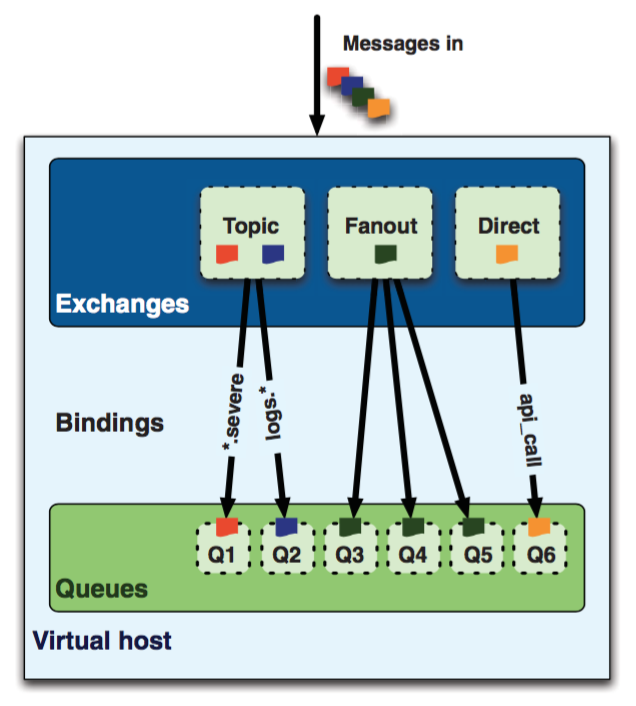
\includegraphics[width=0.3\textwidth]{amqp-stack}
    \caption{Amqp stacks: exchanges, Bindings and Queues}
    \label{fig:amqp-stack}
\end{figure}
Là nơi các message được chứa và chờ được các consumers nhận. Consumers có thể nhận các thông điệp từ queue theo một trong hai cách sau:
\begin{itemize}
	\item Đăng ký nhận thông qua lệnh basic.consume trong AMQP. Lệnh này sẽ tạo kênh (channel) đặt trong chế độ nhận đến khi nào huỷ đăng ký khỏi hàng đợi (queue). Khi subcribe vào một queue, consumber sẽ nhận tự động nhận các thông điệp nếu có từ queue sau khi xử lý xong thông điệp cuối cùng trong queue. Nên sử dụng basic.consume trong trường hợp consumser xử lý nhiều thông điệp một cách tự động ngay sau khi thông điệp này được chuyển tới queue.
	\item Đôi khi chỉ cần có một tin nhắc duy nhất từ hàng đợi mà không yêu cầu phải liên tục, sử dụng lệnh basic.get. 	
\end{itemize}
Nếu có nhiều consumers đăng ký vào cùng một hàng đợi, RabbitMQ sẽ chỉ chuyển thông điệp đến cho một hàng đợi theo cơ chế round-robin. 
\newline
Nếu sử dụng cơ chế auto-ack, thì khi consumer nhận được thông điệp từ queue sẽ phải gửi lại cho RabbitMQ một acknowledge message để  RabbitMQ biết là thông điệp đó đã được nhận và remove khỏi queue. Trong trường hợp consumer nhận thông điệp và mất kết nối tới RabbitMQ, RabbitMQ sẽ coi thông điệp đó vẫn chưa được gửi đi và sẽ vẫn lưu lại ở queue để phân phát cho consumer mới đăng ký.
\newline
Một số thuộc tính hay dùng cho queue:
\begin{itemize}
	\item exclusive: nếu set là true thì queue là private, chỉ được consume bởi một ứng dụng duy nhất. Nên dùng khi muốn hạn chế một queue chỉ được duy nhất một consumer.
	\item auto-delete: queue sẽ tự động delete khi queue không có consumer nào đăng ký nhận message. Nếu cần một queue tạm để cho duy nhất một consumer có thể kết hợp exclusive và auto-delete.
\end{itemize}

\subsubsection{Exhanges và bindings}
Bất cứ khi nào bạn muốn phân phát message tới queue, thì phải gửi message vào một exchange. Một queue sẽ được gắn (binding) vào exchange bởi một routing key. Exchange sẽ dựa vào routing-key để quyết định queue nào sẽ được phân phát message. Các loại exchanges: 

\paragraph{Direct exchange:} sẽ phân phát các thông điệp tới các hàng đợi dựa vào routing key. Routing key là một thuộc tính của thông điệp được gán vào trong header của thông điệp khi producer gửi thông điệp. Thông điệp được gửi đến một hàng đợi mà có routing key trùng với routing key của thông điệp (Hình \ref{fig:directExchange}). Trường hợp sử dụng:
\begin{itemize}
  \item Direct exchange được sử dụng trong định tuyến đơn hướng thông điệp.
  \item Direct exchange được sử dụng để phân phối nhiệm vụ giữa nhiều workers theo kiểu round robin (luân chuyển). Việc cân bằng tải này được hiểu giữa các consumers chứ không phải giữa các hàng đợi.
\end{itemize}

\begin{figure}[h]
    \centering
    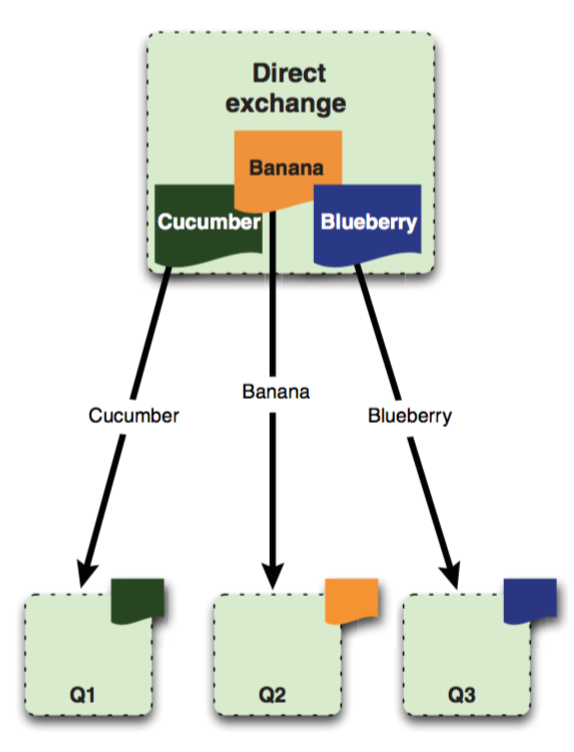
\includegraphics[width=0.3\textwidth]{direct-exchange}
    \caption{Direct exchange message flow}
    \label{fig:directExchange}
\end{figure}


\paragraph{Topic exchange:} sẽ định tuyến thông điệp đến hàng đợi có routing key trùng hoặc gần đúng mẫu routing key của thông điệp. Do đó, thông điệp được gửi đến một hoặc nhiều hàng đợi có routing key trùng hoặc gần đúng mẫu. Ví dụ về routing key: \textit{agreements.us}, \textit{agreements.eu.stockholm} hoặc theo mẫu \textit{agreements.*.*.b.*} - chỉ chấp nhận routing key với từ bắt đầu là \textbf{agreements} và từ thứ 4 là \textbf{b}; \textit{agreements.eu.berlin.\#} - chấp nhận routing key bắt đầu bằng \textbf{agreements.eu.berlin} (Hình \ref{fig:topicExchange}). Bất cứ khi nào một vấn đề liên quan đến nhiều consumers/appications có chọn lọc loại thông điệp muốn nhận, topic exchange là lựa chọn phù hợp. Một số ca sử dụng thường gặp: 
\begin{itemize}
	\item Phân phối các dữ liệu có liên quan đến vị trí địa lý cụ thể, ví dụ, các điểm bán hàng.
	\item Cập nhật tin tức liên quan đến việc phân loại và gắn nhãn (ví dụ, chỉ cho một môn thể thao hoặc nhóm cụ thể).
	\item Cập nhật giá cổ phiếu (và cập nhật về các loại dữ liệu tài chính).
\end{itemize}
\begin{figure}[h]
    \centering
    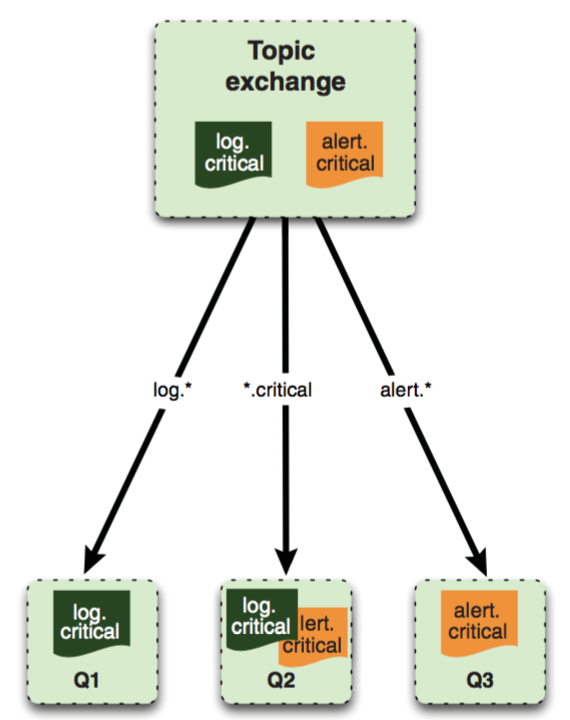
\includegraphics[width=0.3\textwidth]{topic-exchange}
    \caption{Topic exchange message flow}
    \label{fig:topicExchange}
\end{figure}

\paragraph{Fanout exchange:} sao chép và phân phát tất cả thông điệp đến tất cả hàng đợi được gán vào exchange mà không cần quan tâm đến routing key như direct hoặc topic exchange. Fanout exchange được sử dụng trong trường hợp cùng một thông điệp cần gửi đến một hoặc nhiều hàng đợi với nhiều consumers xử lý thông điệp theo những cách hác nhau (Hình \ref{fig:fanoutExchange}). Ca sử dụng thường gặp:
\begin{itemize}
	\item Các trang web tin tức thể thao có thể sử dụng để phân phối bản cập nhật điểm cho các khách hàng điện thoại di động trong thời gian gần thực.
	\item Phân phát thông tin cập nhật cổ phiếu cho các ứng dụng như bảng giá, mobile đặt lệnh, vẽ biểu đồ mã chứng khoán thời gian thực.
\end{itemize}
\begin{figure}[h]
    \centering
    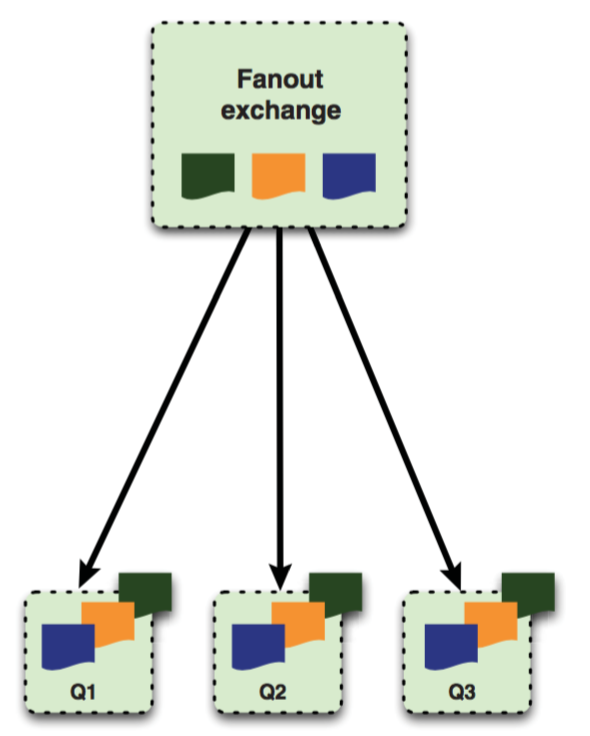
\includegraphics[width=0.3\textwidth]{fanout-exchange}
    \caption{Fanout exchange message flow}
    \label{fig:fanoutExchange}
\end{figure}
\section{Apache ActiveMQ}
\subsection{Định nghĩa}
\subsection{ZeroMQ}
\subsection{Apache Kafka}
\end{document}